\section{Testing the Implementation}

In this chapter the algorithm described in chapter \ref{implement} will be used to generate undistorted images from at least four different images from each recording.\\

Additionally the calculated intrinsic matrix $I$ and the calculated distortion coefficient vector $d$ will be presented to the individual recordings. The Matrix  and the coefficients have the following form:\\
\vspace{-6mm}
\begin{center}
\hspace{10mm}\textbf{Intrinsic Matrix}
\end{center}
\begin{equation*}
I =
    \begin{pmatrix}
     f \cdot k_1 & -k_1/tan(\theta)) & s_1\\ 
     0 & f \cdot k_2/sin(\theta) & s_2\\ 
     0 & 0 & 1
    \end{pmatrix}
\end{equation*}
where
\begin{tabular}[t]{ll}
    $f$ & Focal length in mm\\
    $k_1$ & Resolution of image sensor in Z1 direction in pixel per mm\\
    $k_2$ & Resolution of image sensor in Z2 direction  in m/s\\
    $s_1$ & Offset between optical centre and image origin in Z1 in mm\\
    $s_2$ & Offset between optical centre and image origin in Z2 in mm\\
    $\theta$ & Shearing angle of the image axes\\
\end{tabular}
\vspace{5mm}

\begin{center}
\hspace{10mm}\textbf{Distortion coefficients}
\end{center}
\vspace{-2mm}
\begin{equation*}
\hspace{10mm}d =
    \left ( k_1, k_2, p_1, p_2, k_3 \right )^{T}
\end{equation*}
where
\begin{tabular}[t]{ll}
    $k_n$ & First $n$ radial distortion terms\\
    $p_n$ & Tangential distortion coefficients \cite{mat_calib}\\
\end{tabular}

\newpage

\begin{itemize}[leftmargin=*]
    \item \textbf{\large Recording of checkerboard\_000.h264}
\end{itemize}
The recording \textit{checkerboard\_000.h264} was run through with the pipelines described in chapter \ref{implement} with a corner size of 7x7. In the process 10 checkerboards there successfully found and used for the calculation of the intrinsic matrix and the distortion coefficients. The intrinsic matrix and the distortion coefficients are as follows:

\vspace{1mm}
\begin{equation*}
    K_1 = 
    \begin{pmatrix}
        1251.51 & 0 & 924.7\\
        0 & 1252.07 & 451.81\\
        0 & 0 & 1\\
    \end{pmatrix}
\end{equation*}
\vspace{1mm}
\begin{equation*}
    d_1 = (-0.34085, 0.13159, -0.00068, -0.00167, -0.02493)
\end{equation*}

In figure \ref{fig:rec_000} one can see four example frames of the recording which there undistorted:

\begin{figure}[H]
     \centering
     \captionsetup{justification=centering}
     \begin{minipage}[t]{0.24\textwidth}
        \centering
        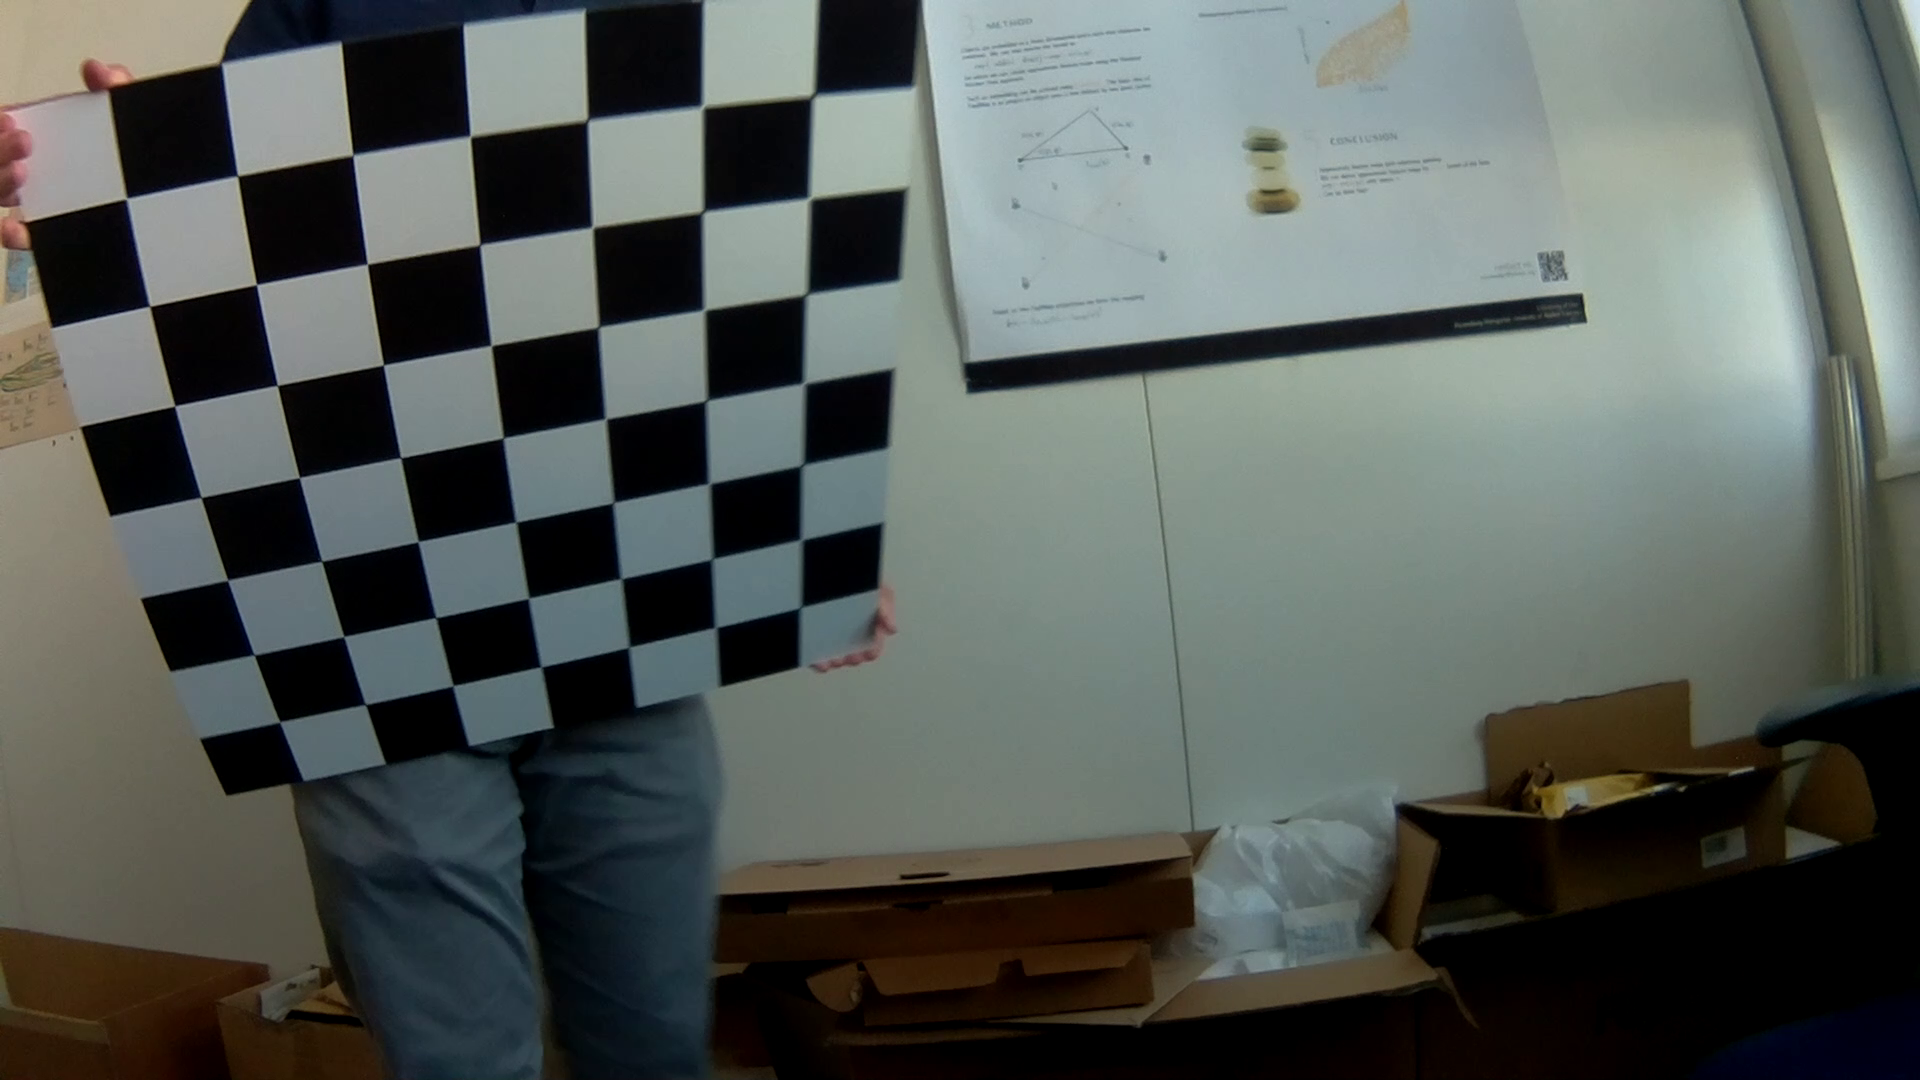
\includegraphics[width=.95\textwidth]{image/3/rec_1/931_og.png}
     \end{minipage}%
     \begin{minipage}[t]{0.24\textwidth}
        \centering
        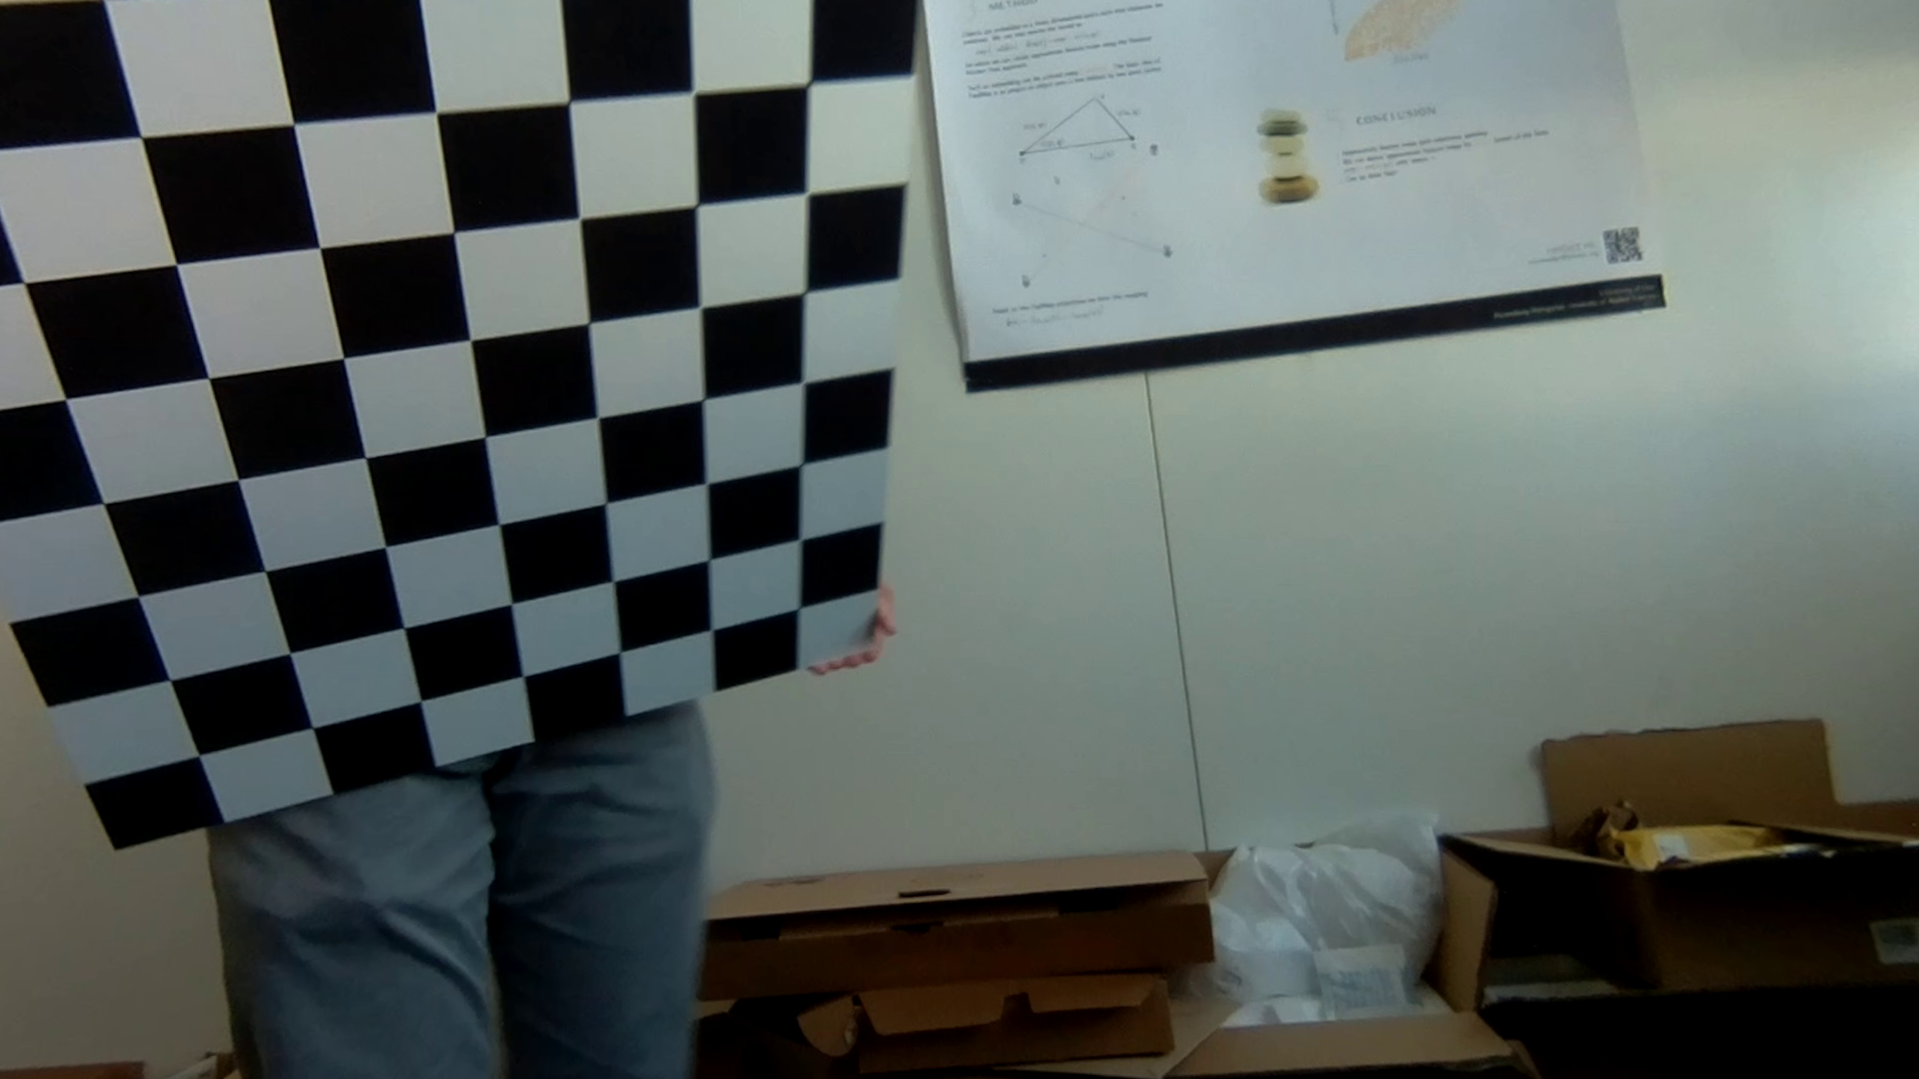
\includegraphics[width=.95\textwidth]{image/3/rec_1/931_undist.png}
     \end{minipage}
     \begin{minipage}[t]{0.24\textwidth}
        \centering
        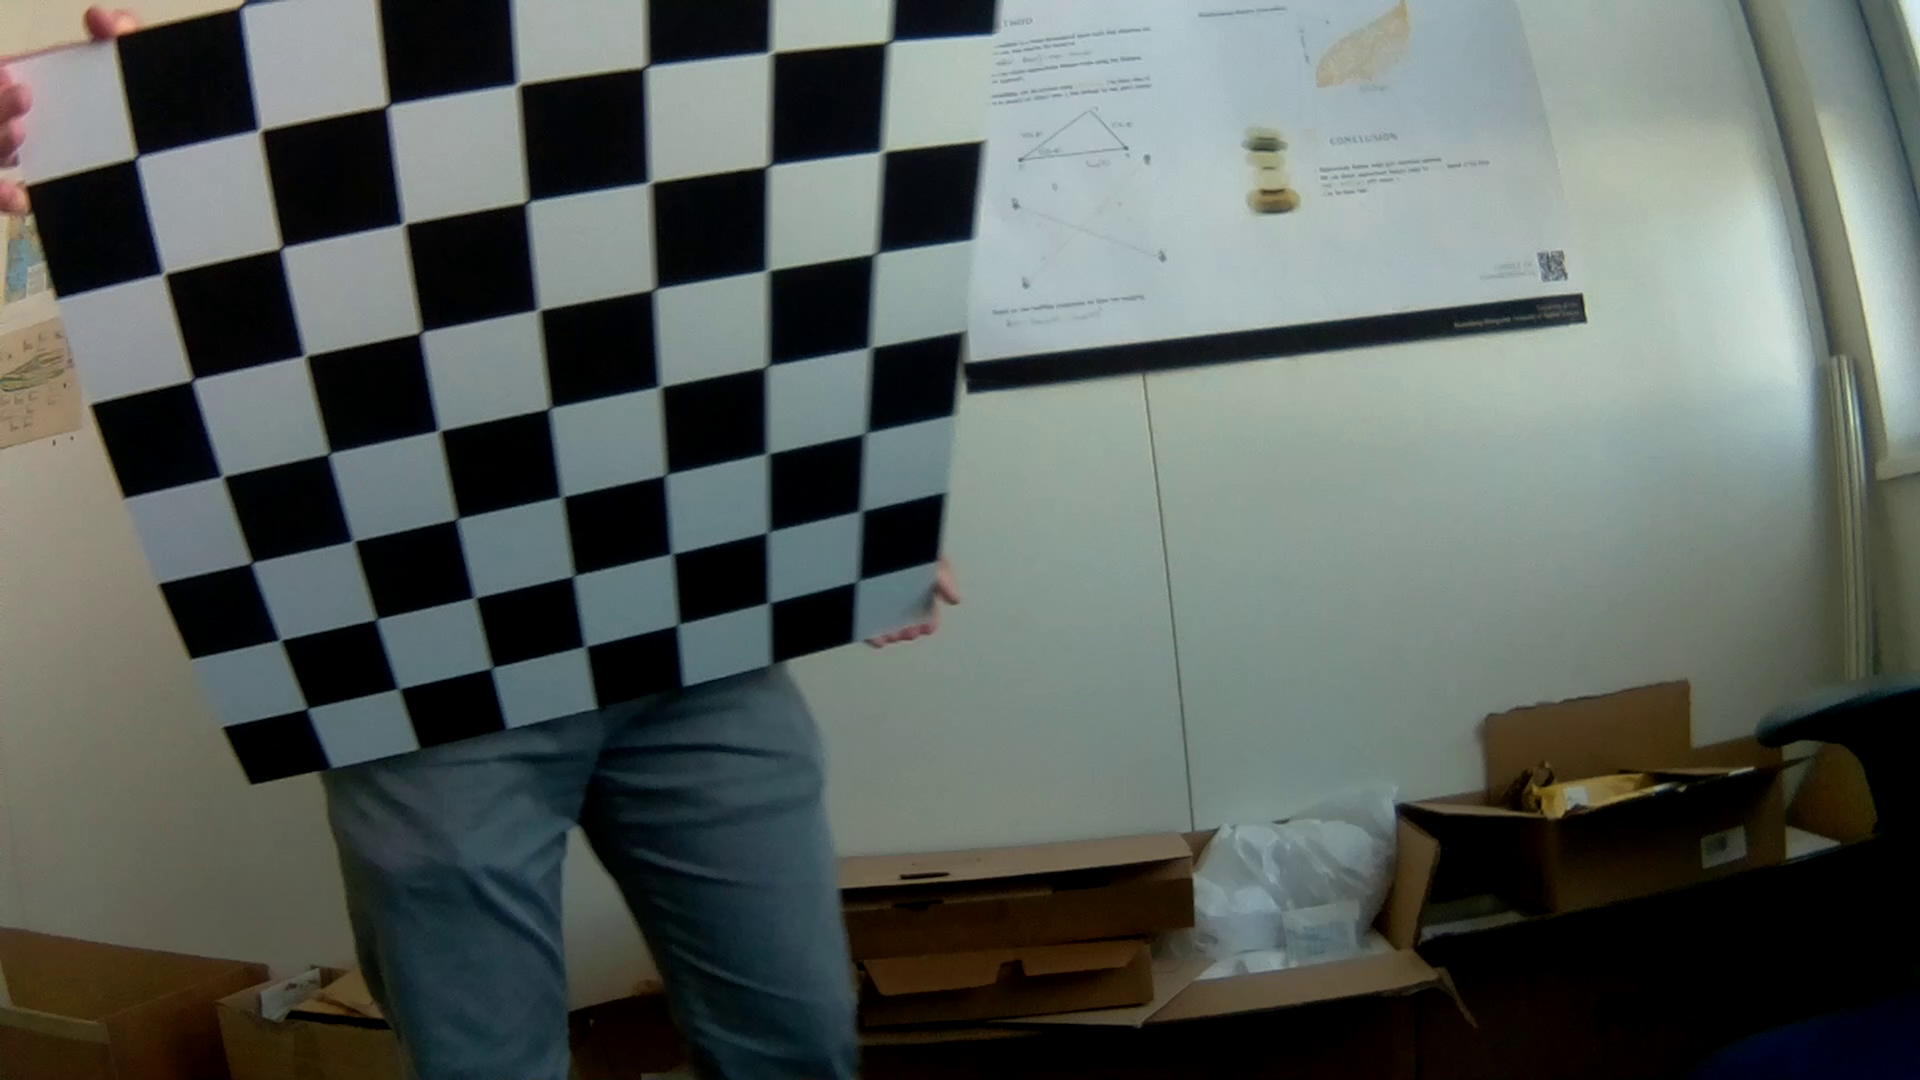
\includegraphics[width=.95\textwidth]{image/3/rec_1/940_og.png}
     \end{minipage}%
     \begin{minipage}[t]{0.24\textwidth}
        \centering
        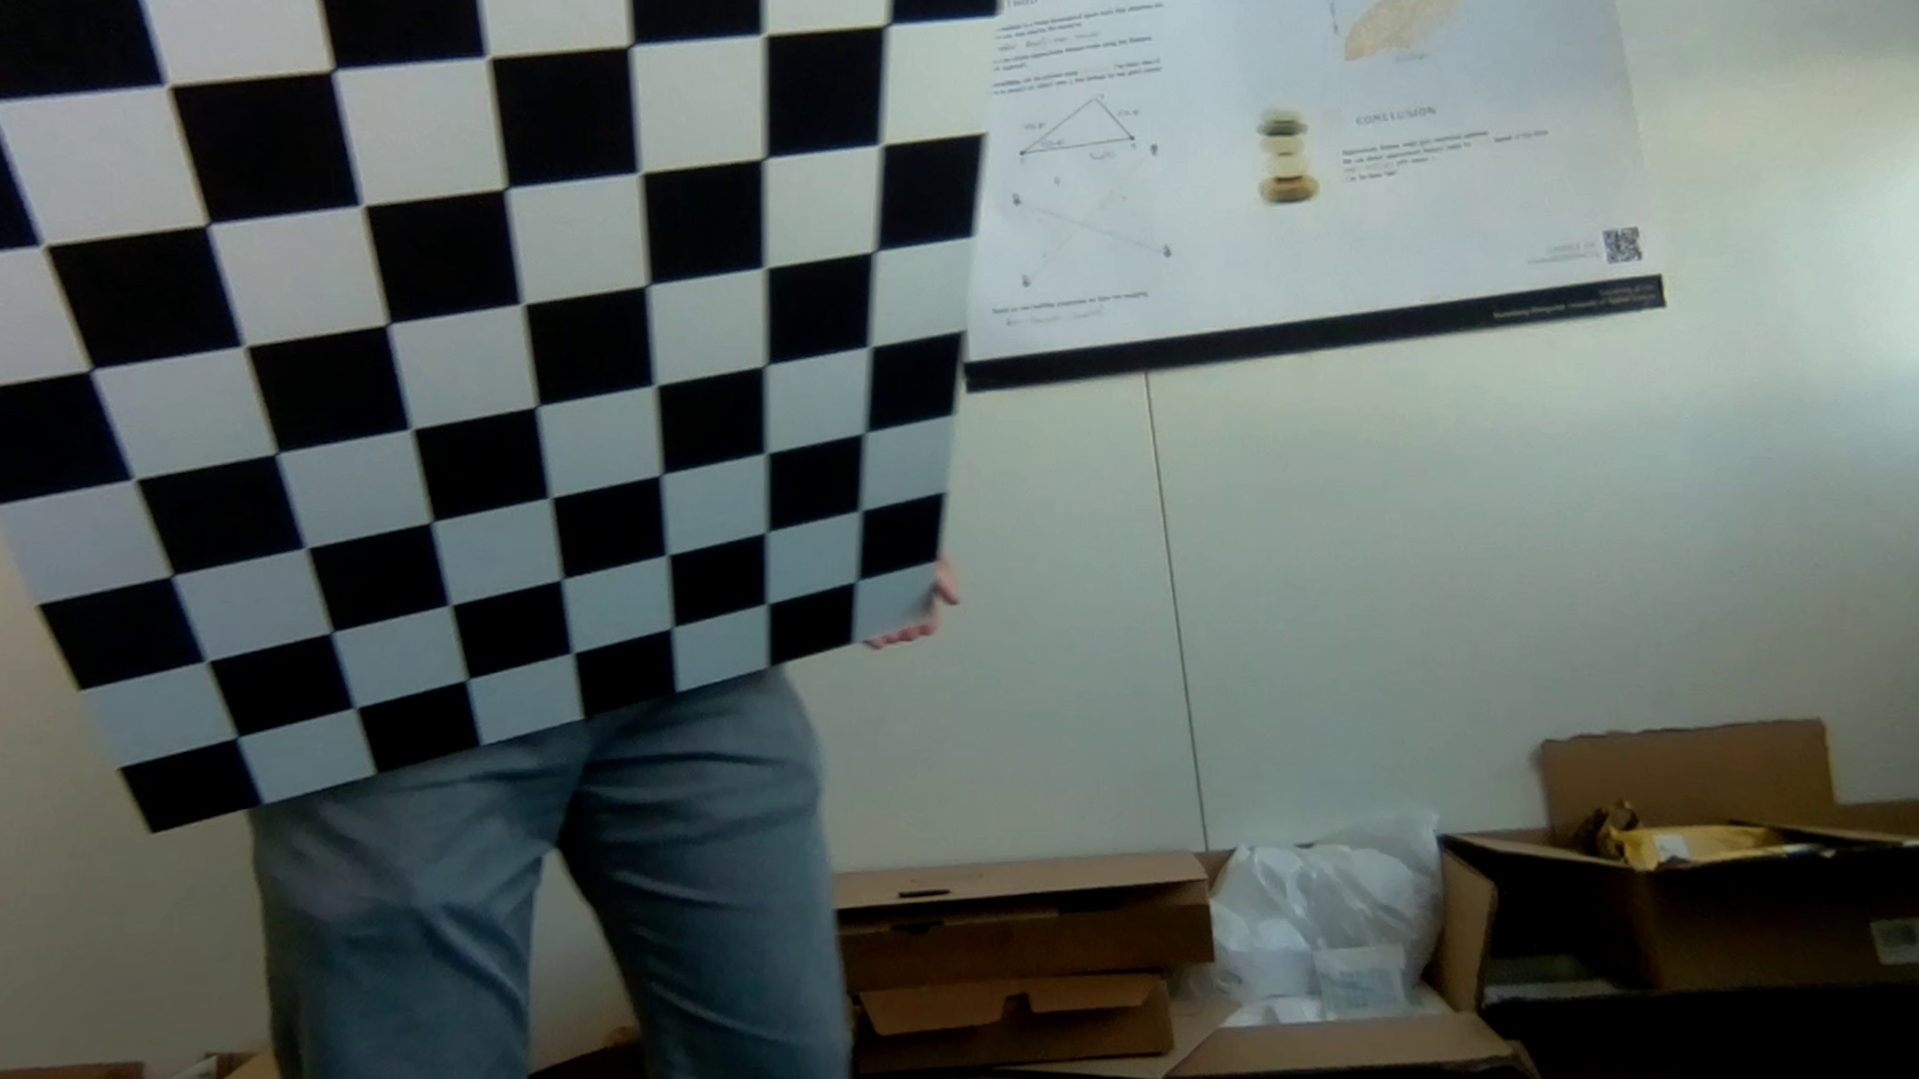
\includegraphics[width=.95\textwidth]{image/3/rec_1/940_undist.png}
     \end{minipage}
     
     \hfill
     
     \begin{minipage}[t]{0.24\textwidth}
        \centering
        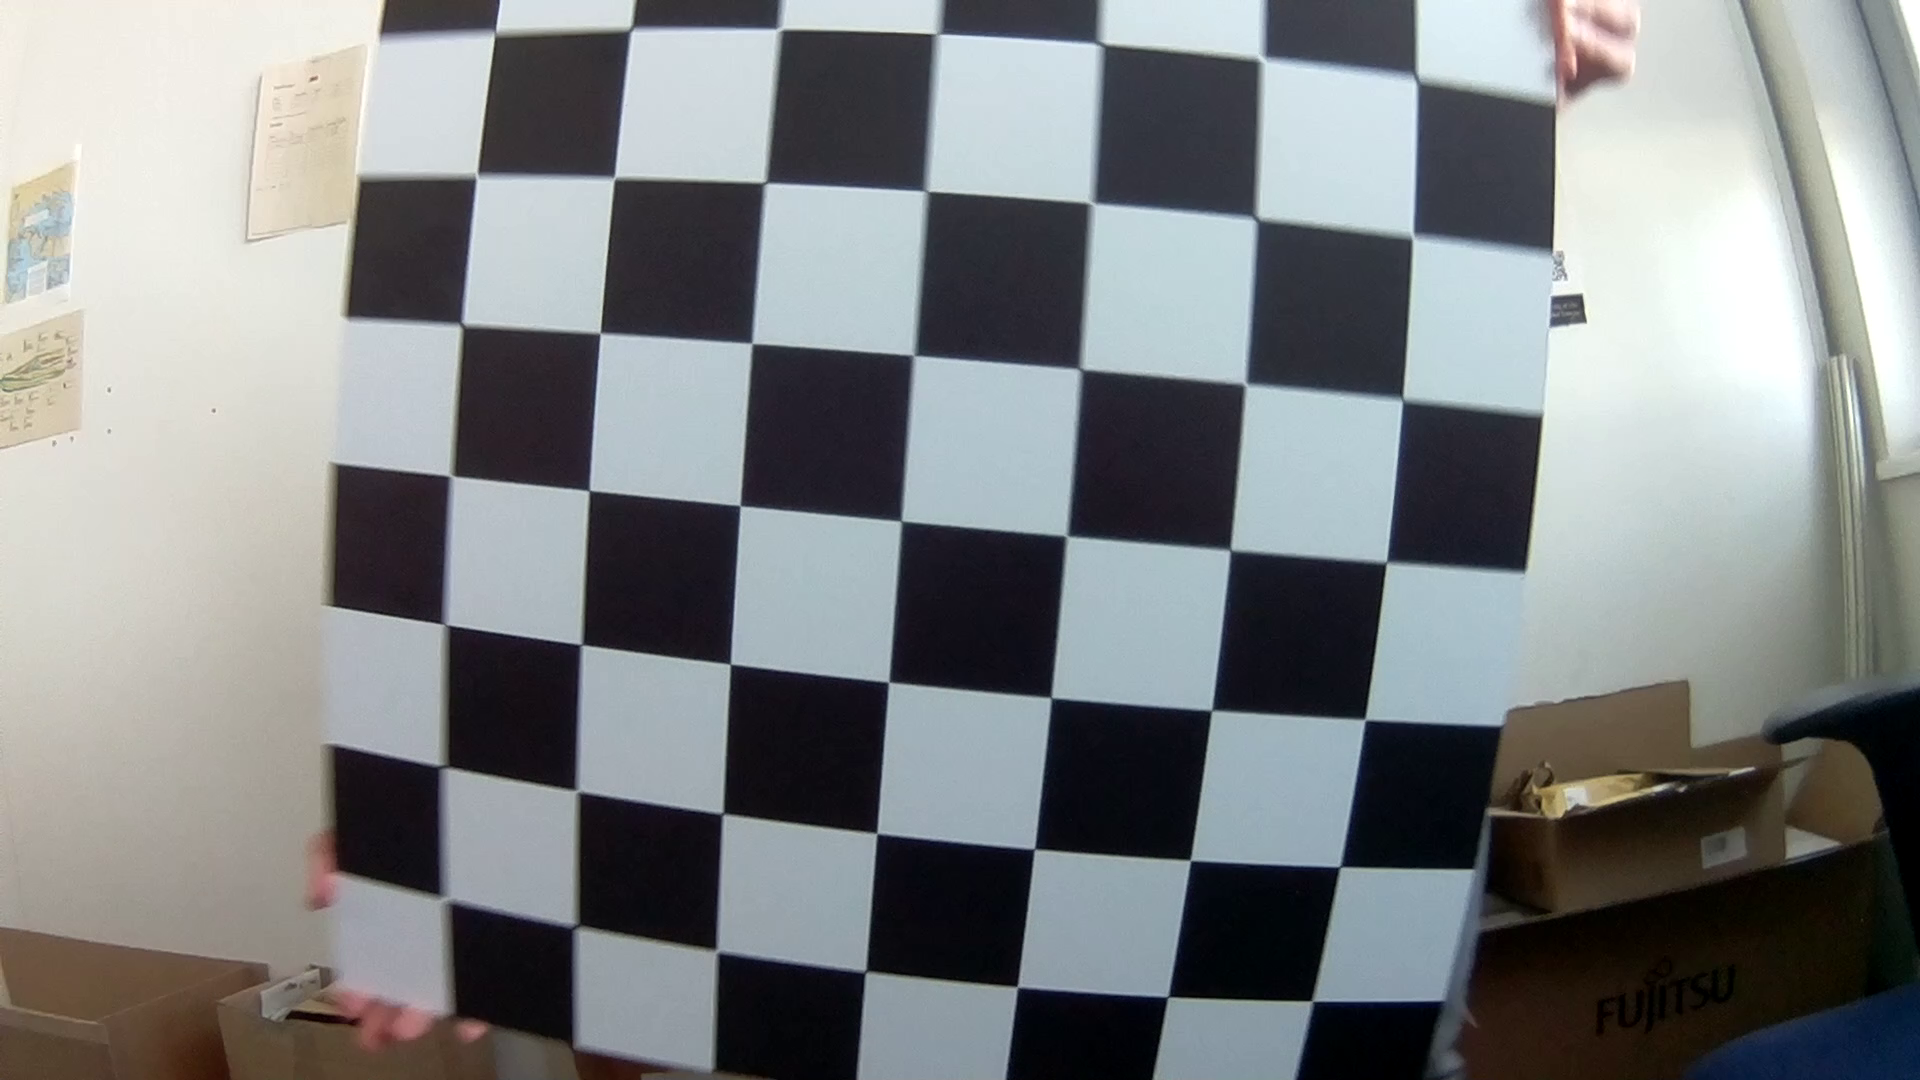
\includegraphics[width=.95\textwidth]{image/3/rec_1/1178_og.png}
     \end{minipage}%
     \begin{minipage}[t]{0.24\textwidth}
        \centering
        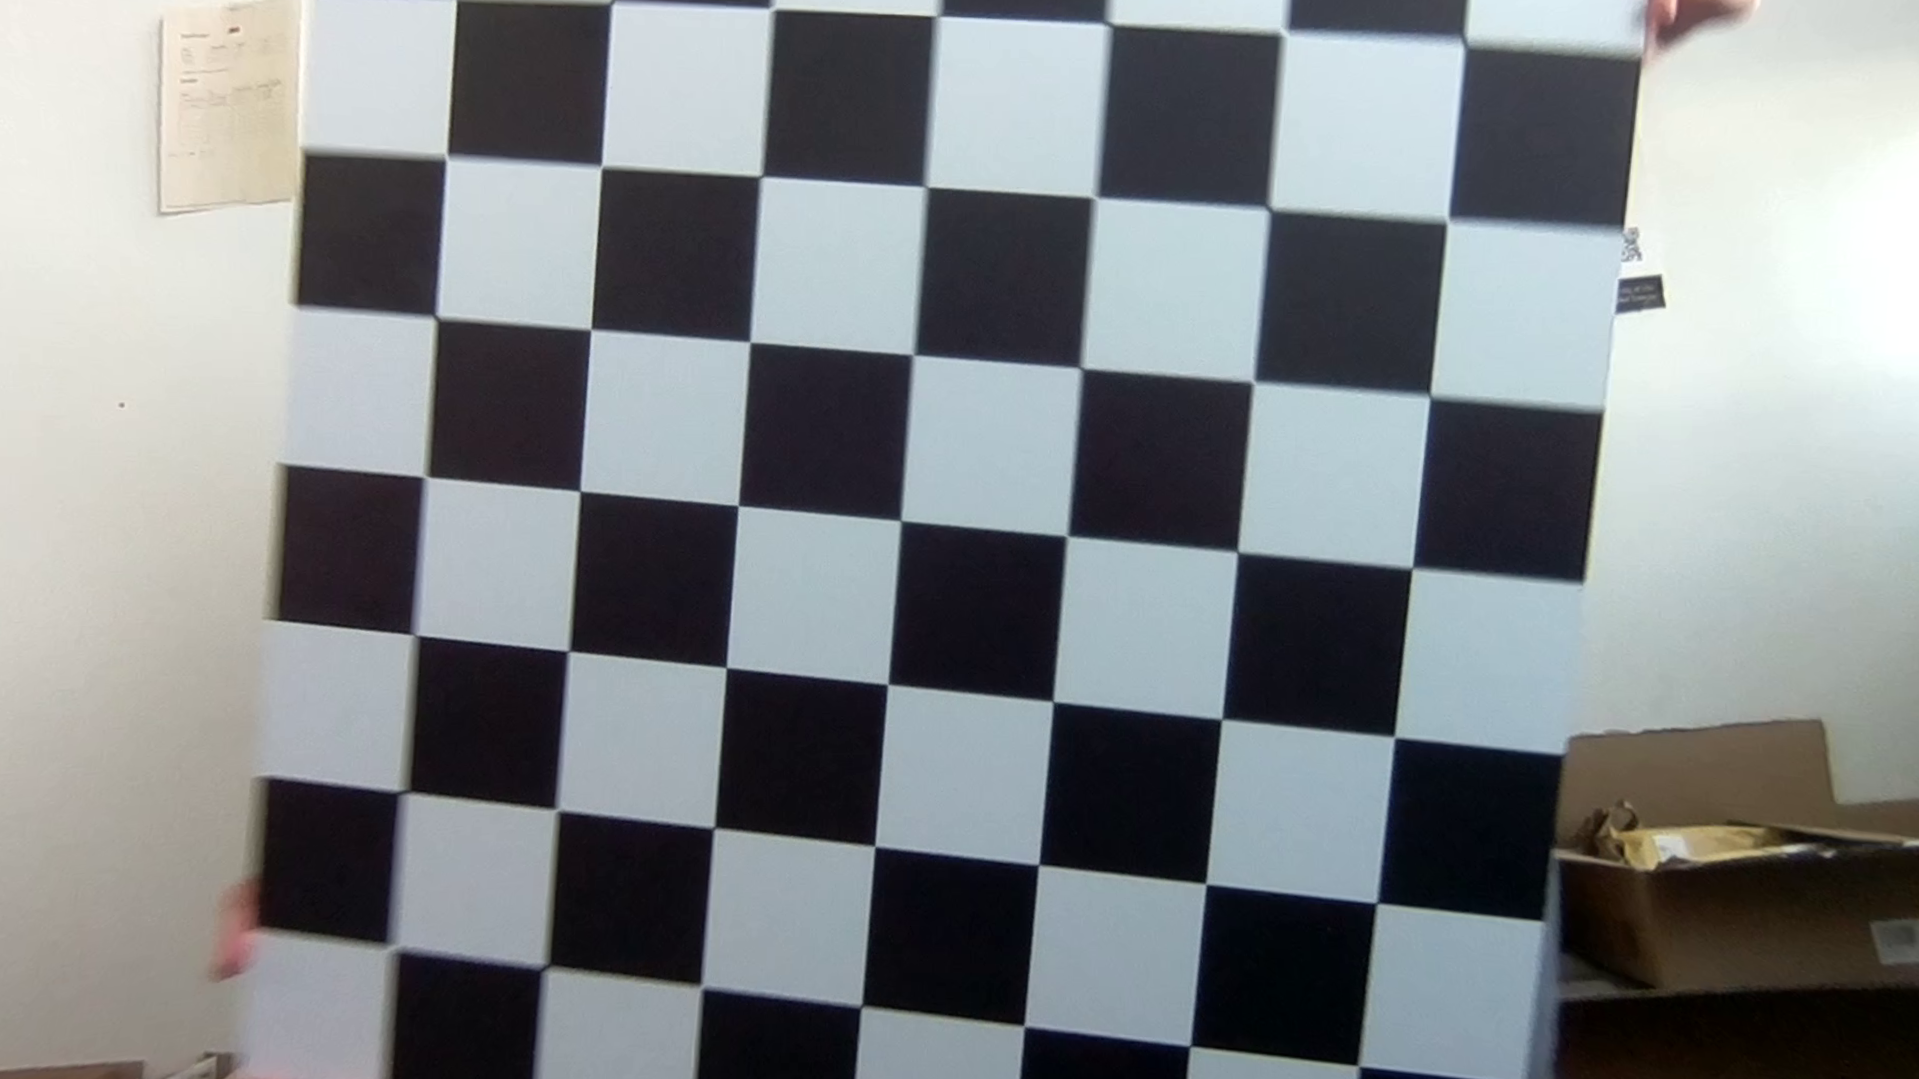
\includegraphics[width=.95\textwidth]{image/3/rec_1/1178_undist.png}
     \end{minipage}
     \begin{minipage}[t]{0.24\textwidth}
        \centering
        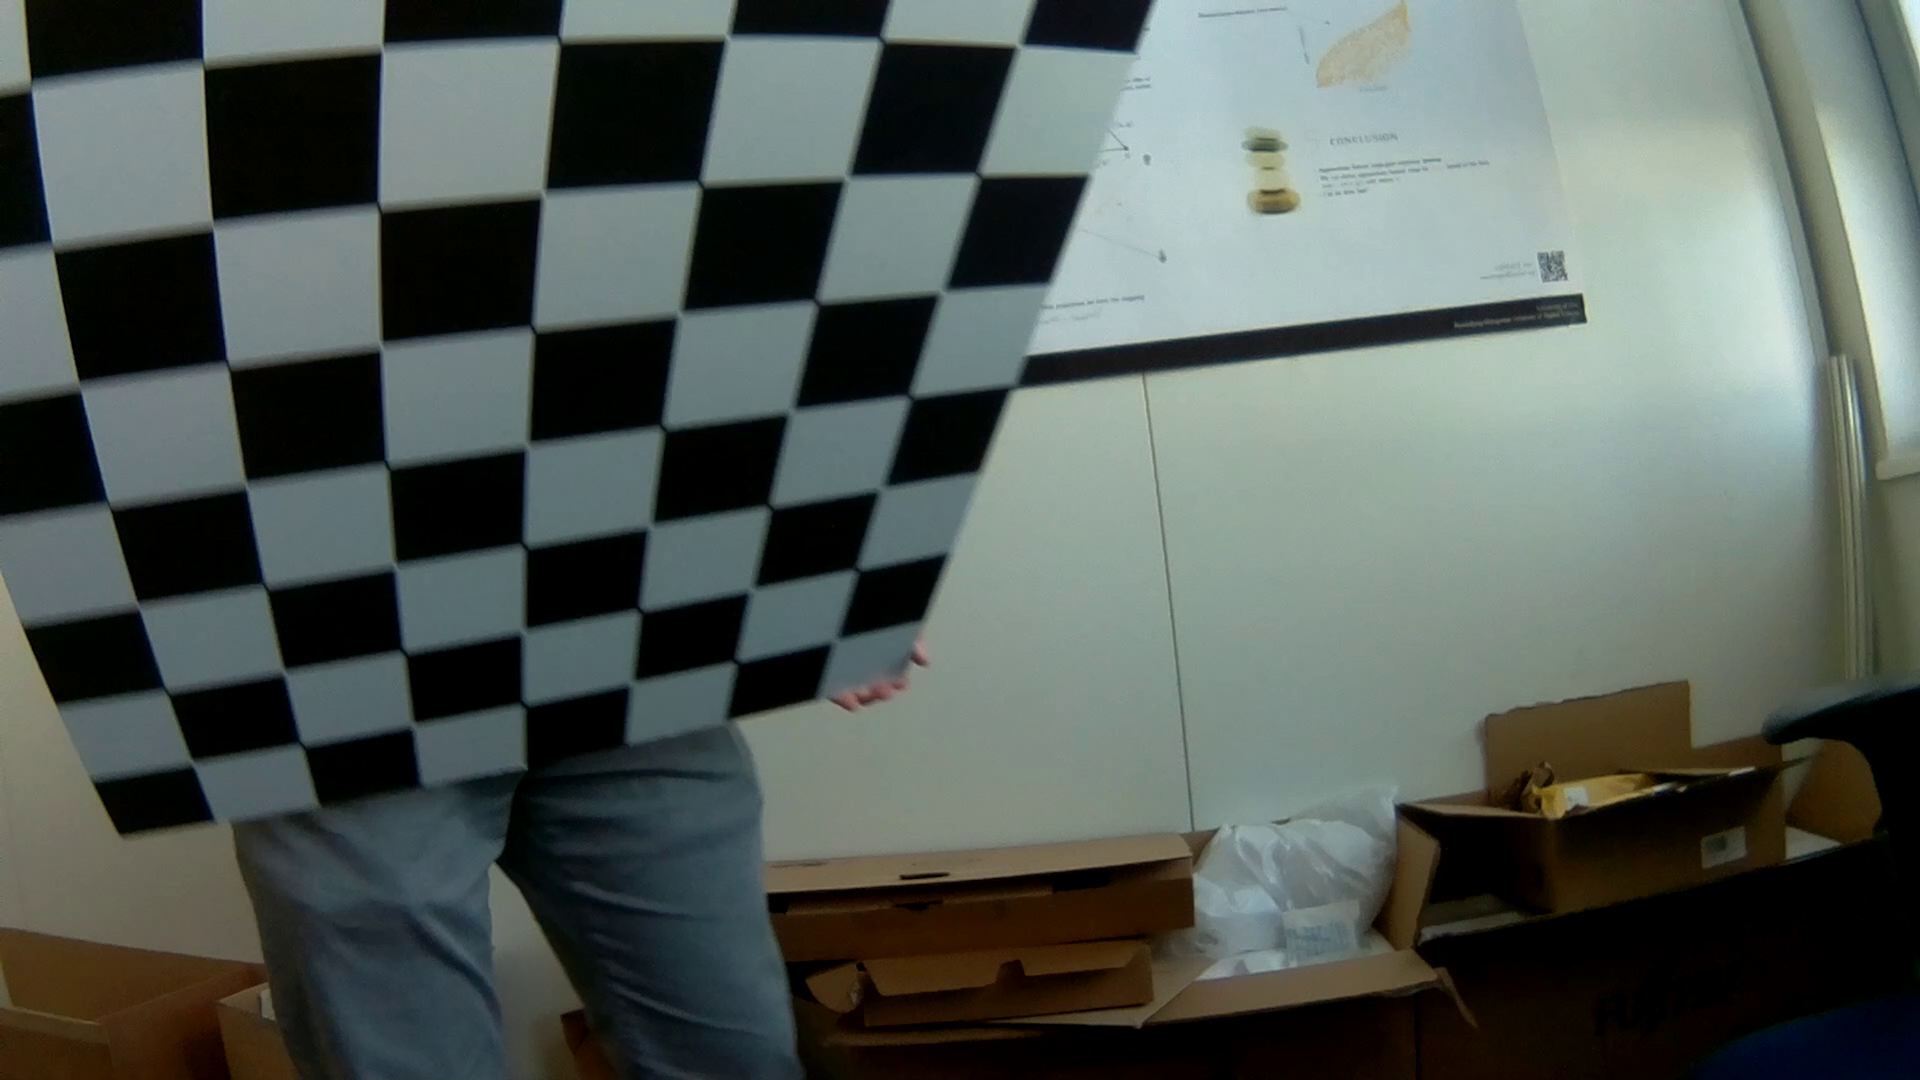
\includegraphics[width=.95\textwidth]{image/3/rec_1/1379_og.png}
     \end{minipage}%
     \begin{minipage}[t]{0.24\textwidth}
        \centering
        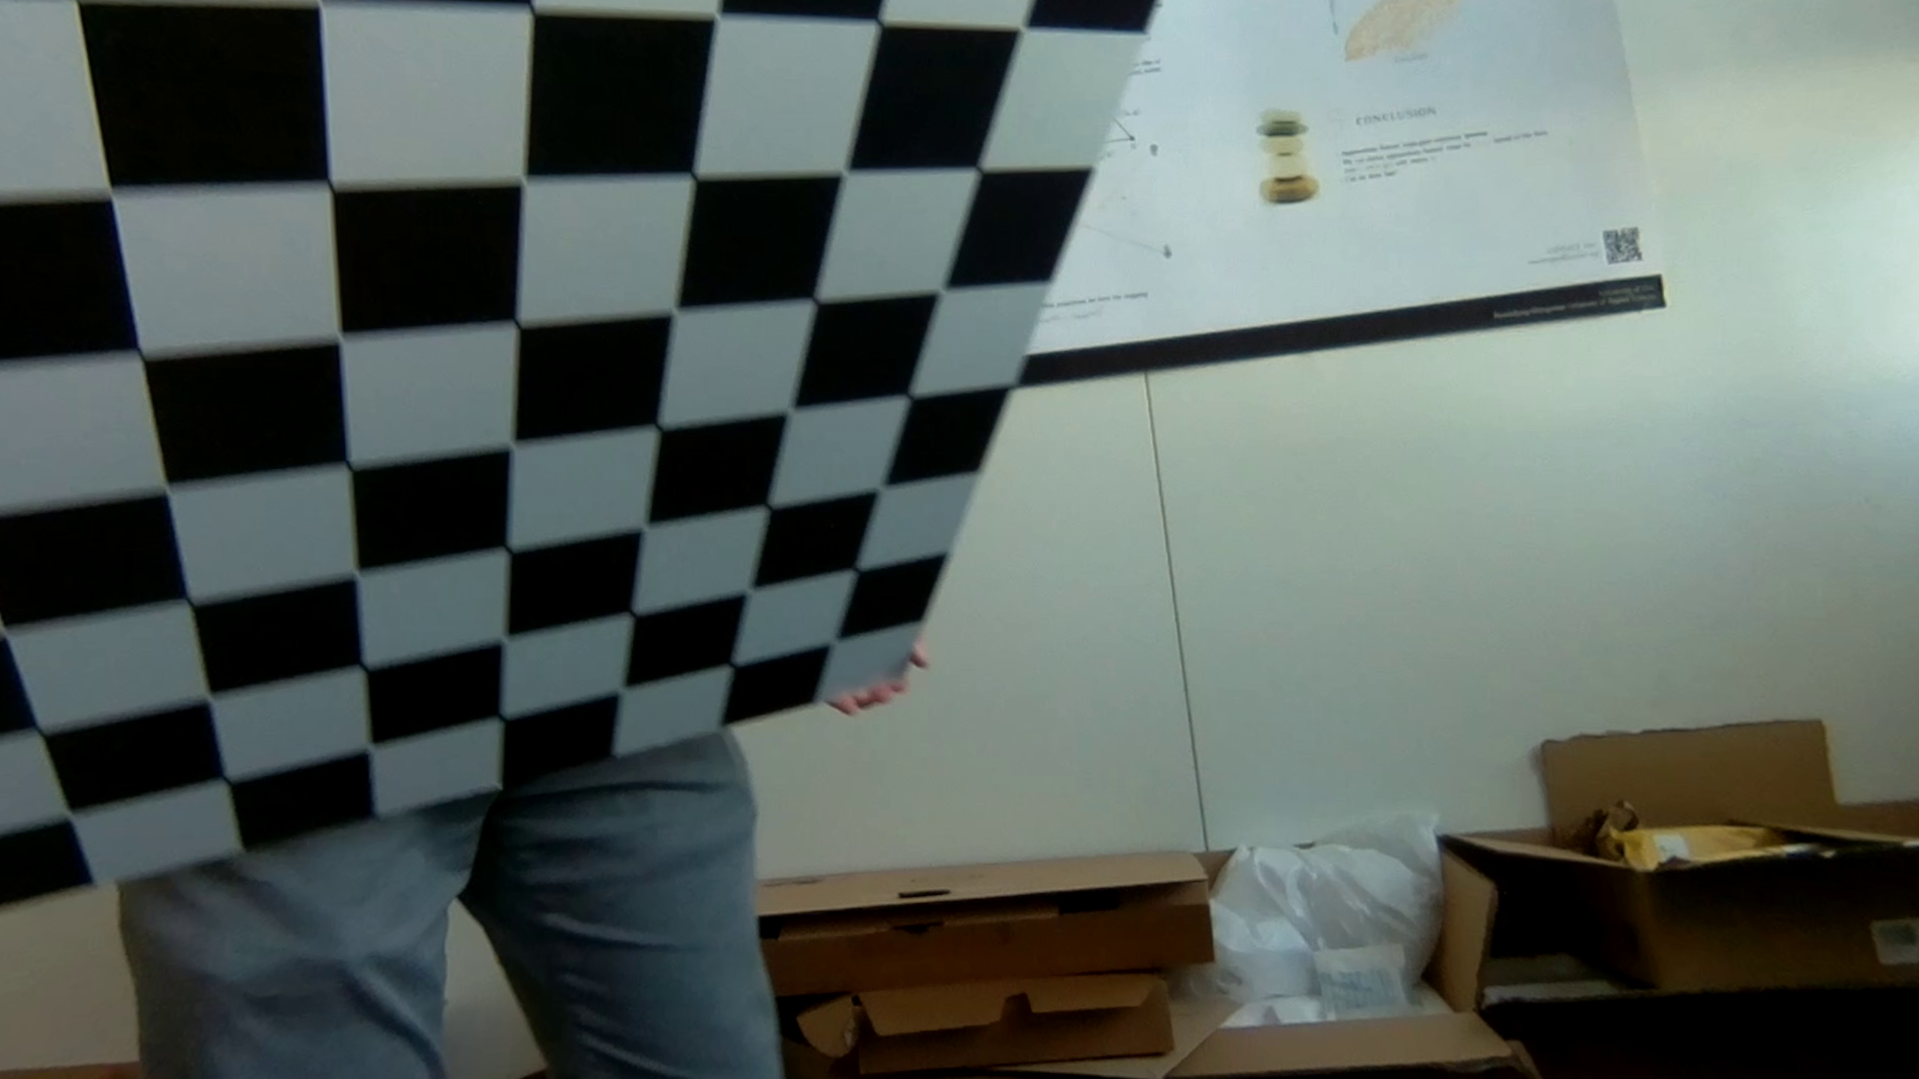
\includegraphics[width=.95\textwidth]{image/3/rec_1/1379_undist.png}
     \end{minipage}
     
     \caption{Four original frames (left) from the recording \textit{checkerboard\_000.h264} with their undistorted counterpart (right)}
    \label{fig:rec_000}
\end{figure}

The undistorted images in figure \ref{fig:rec_000} look like expected: non-straight lines are straightened and most information from the border of the original image is retained. 

\begin{itemize}[leftmargin=*]
    \item \textbf{\large Recording of checkerboard\_019.h264}
\end{itemize}

The recording \textit{checkerboard\_019.h264} was run through with the pipelines described in chapter \ref{implement} with a corner size of 6x6. In the process 71 checkerboards there successfully found and used for the calculation of the intrinsic matrix and the distortion coefficients. The intrinsic matrix and the distortion coefficients are as follows:
\newpage
\begin{equation*}
    K_2 = 
    \begin{pmatrix}
        364.56 & 0 & 1128.71\\
        0 & 363.62 & 622.93\\
        0 & 0 & 1\\
    \end{pmatrix}
\end{equation*}
\vspace{1mm}
\begin{equation*}
    d_2 = (-0.02752, -0.00044, -0.01197, -0.01460, 0.00006)
\end{equation*}

In figure \ref{fig:rec_019} one can see four example frames of the recording which there undistorted:


\begin{figure}[H]
     \centering
     \captionsetup{justification=centering}
     \begin{minipage}[t]{0.24\textwidth}
        \centering
        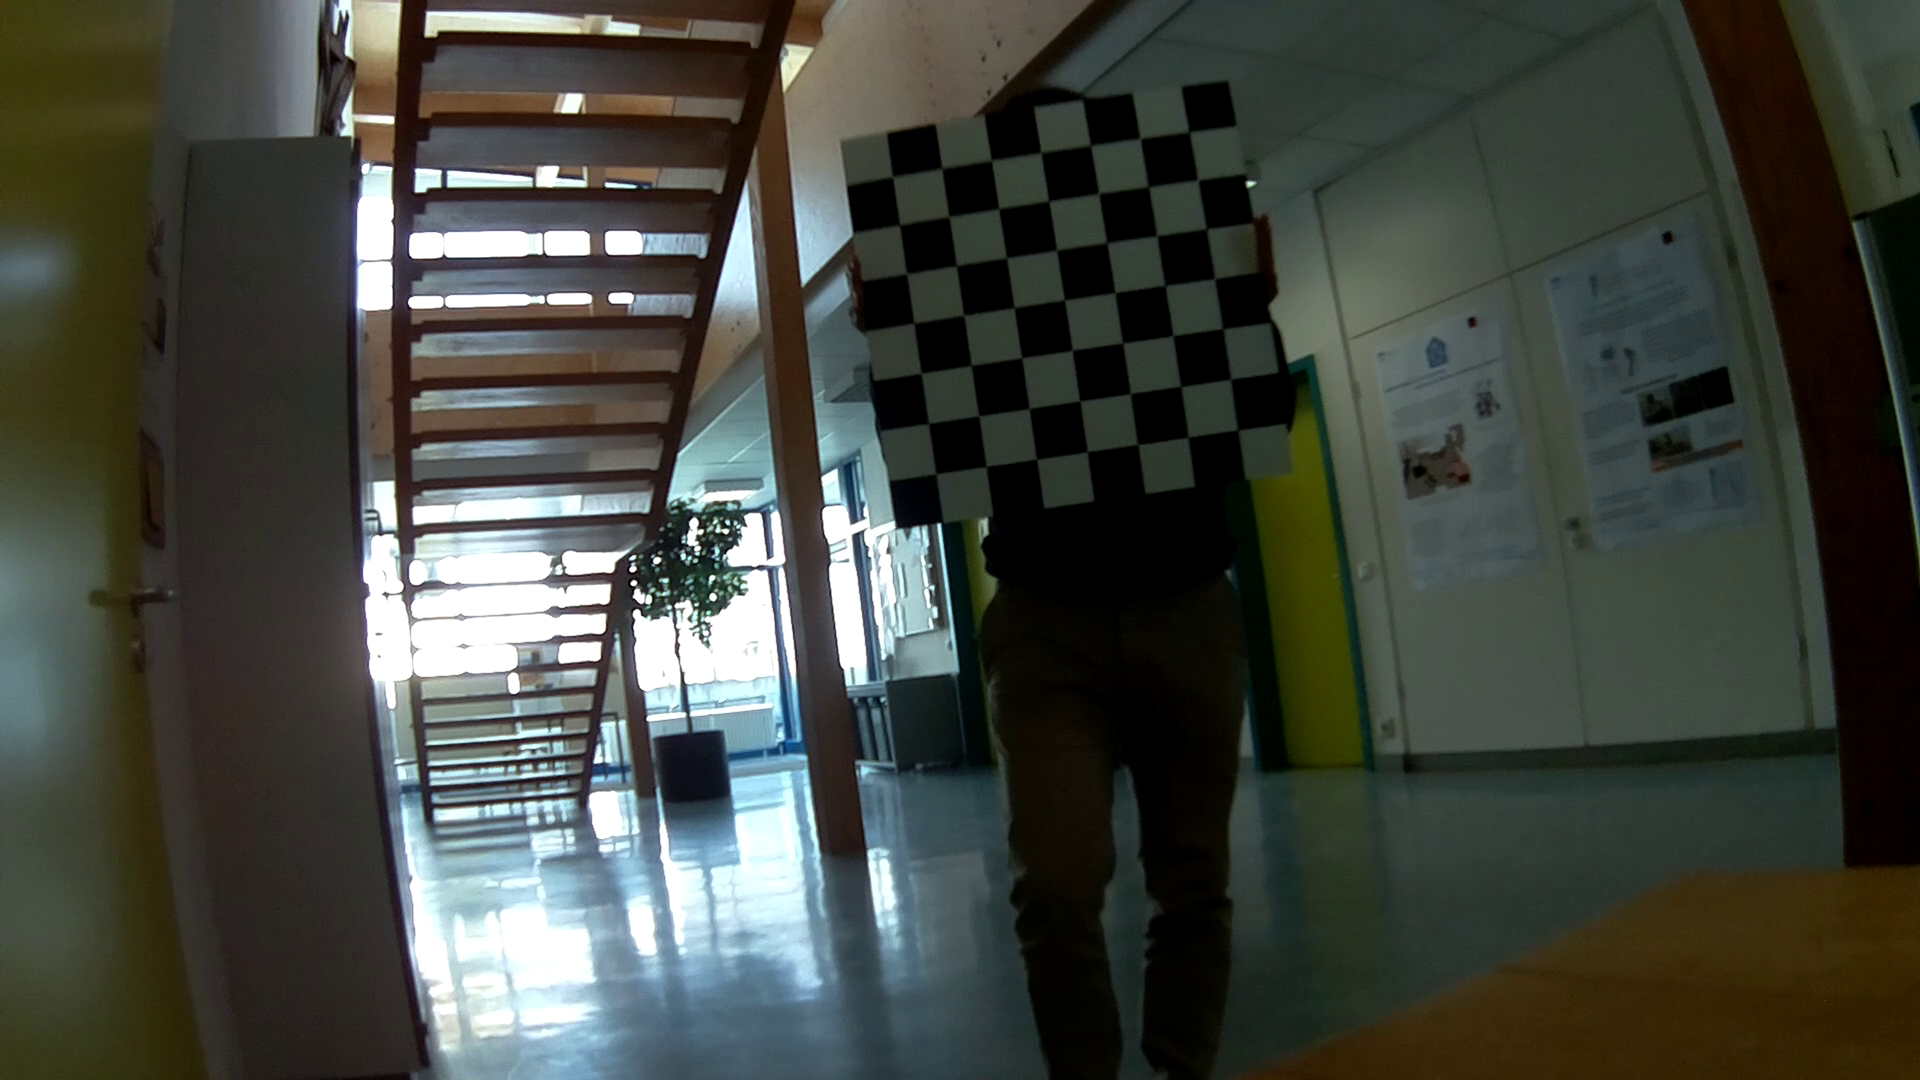
\includegraphics[width=.95\textwidth]{image/3/rec_2/133_og.png}
     \end{minipage}%
     \begin{minipage}[t]{0.24\textwidth}
        \centering
        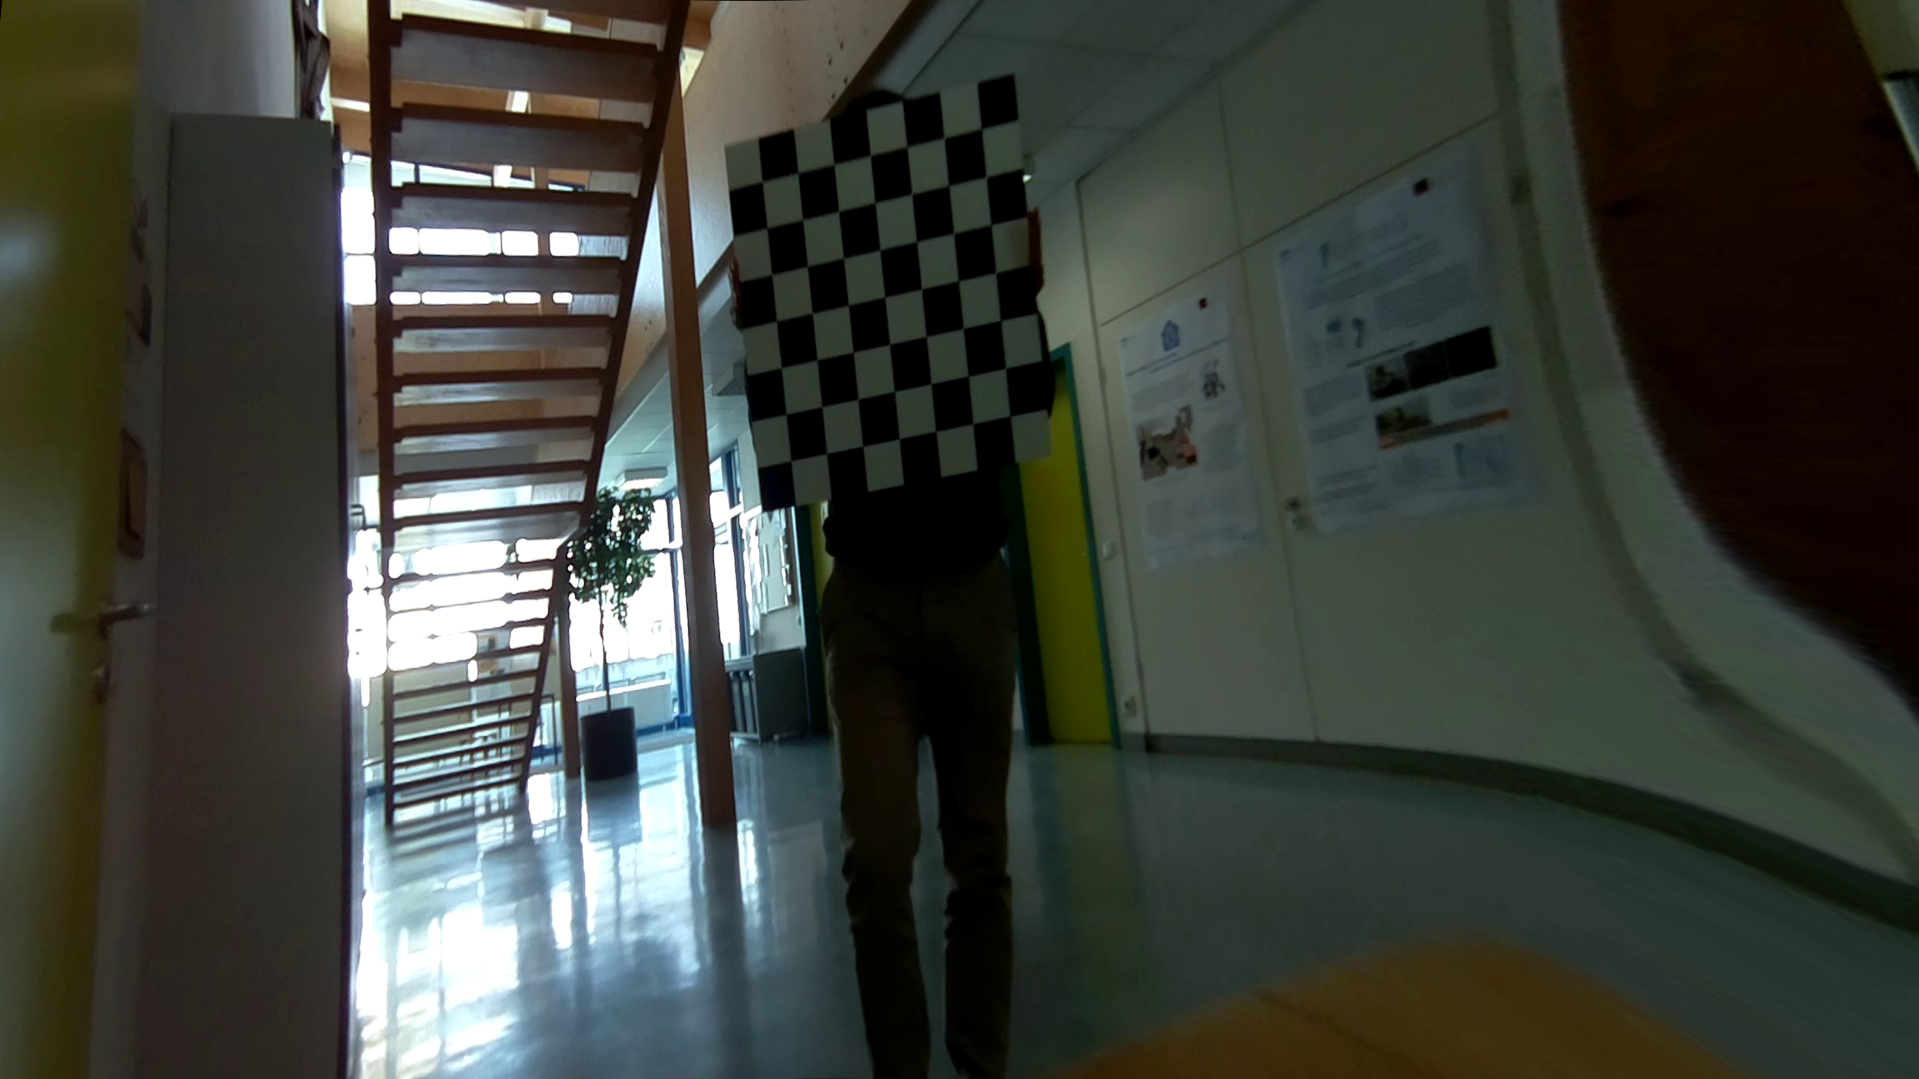
\includegraphics[width=.95\textwidth]{image/3/rec_2/133_undist.png}
     \end{minipage}
     \begin{minipage}[t]{0.24\textwidth}
        \centering
        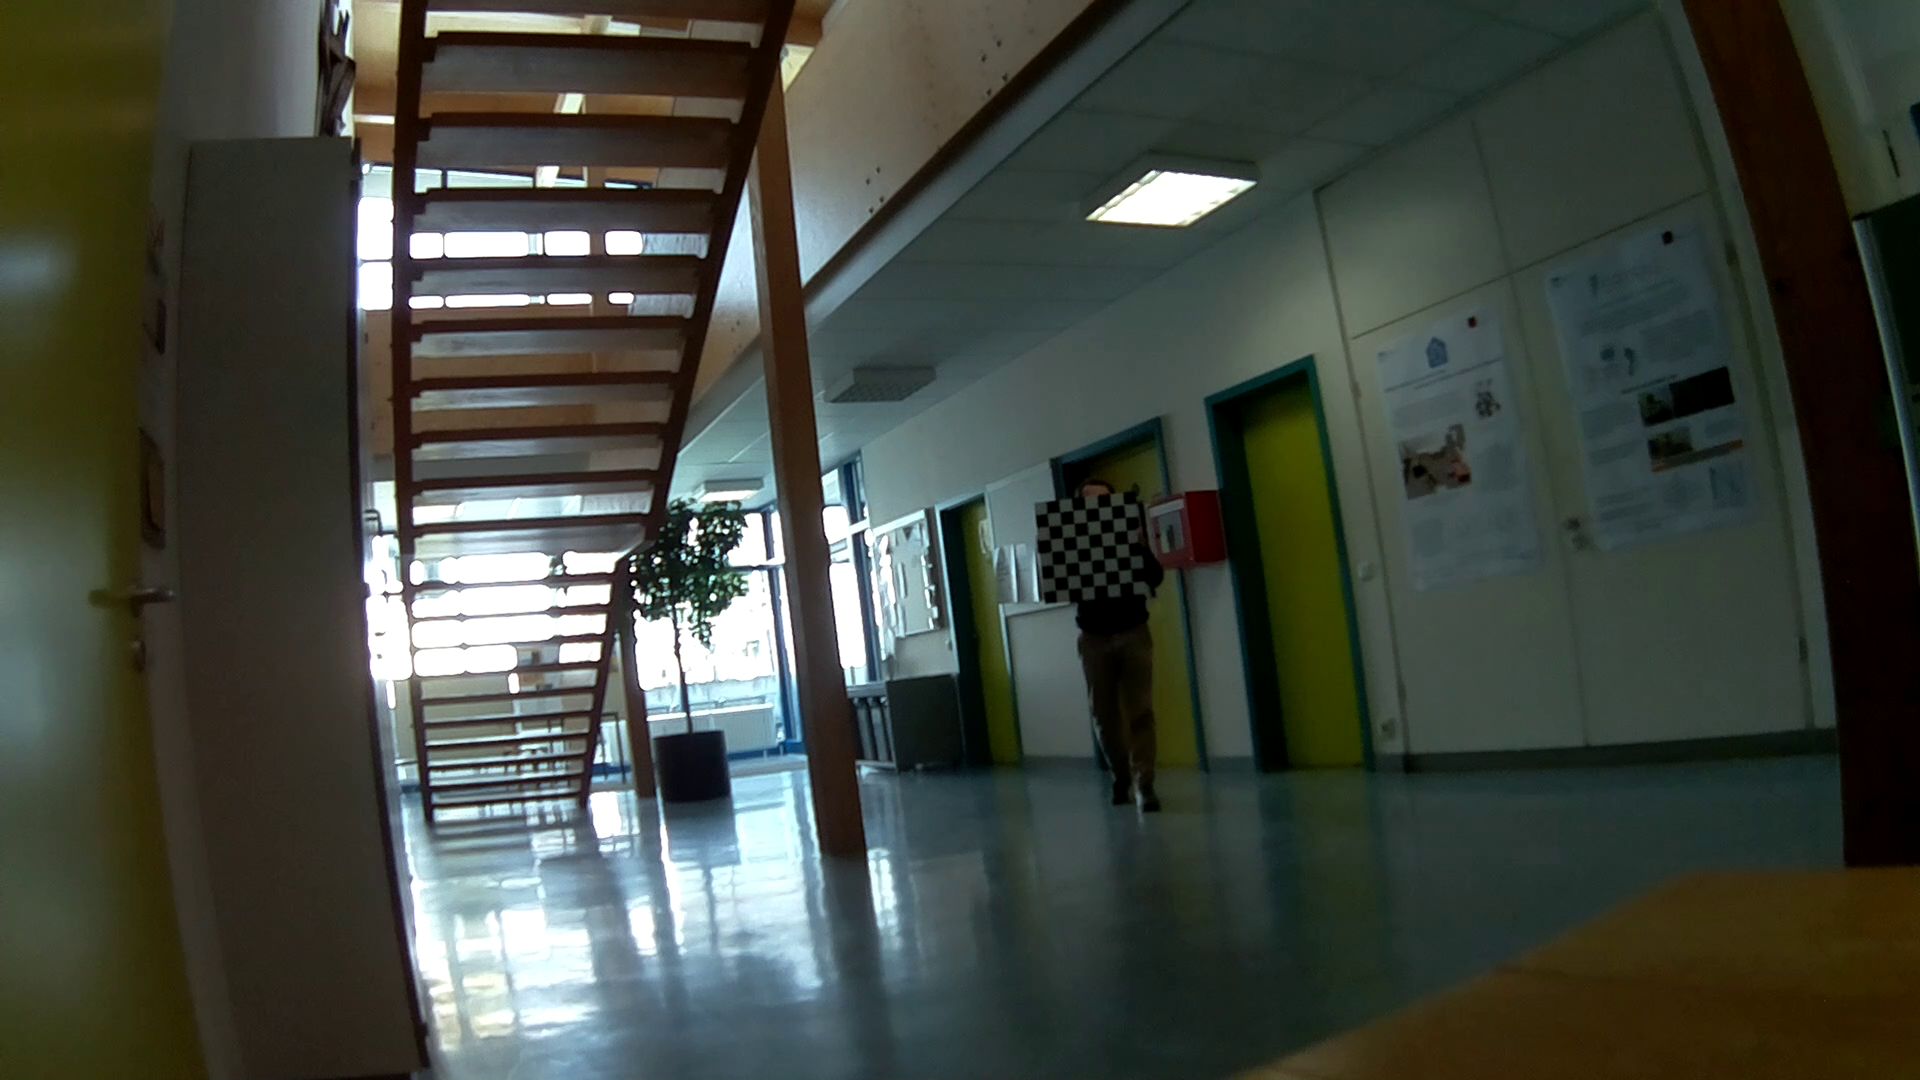
\includegraphics[width=.95\textwidth]{image/3/rec_2/525_og.png}
     \end{minipage}%
     \begin{minipage}[t]{0.24\textwidth}
        \centering
        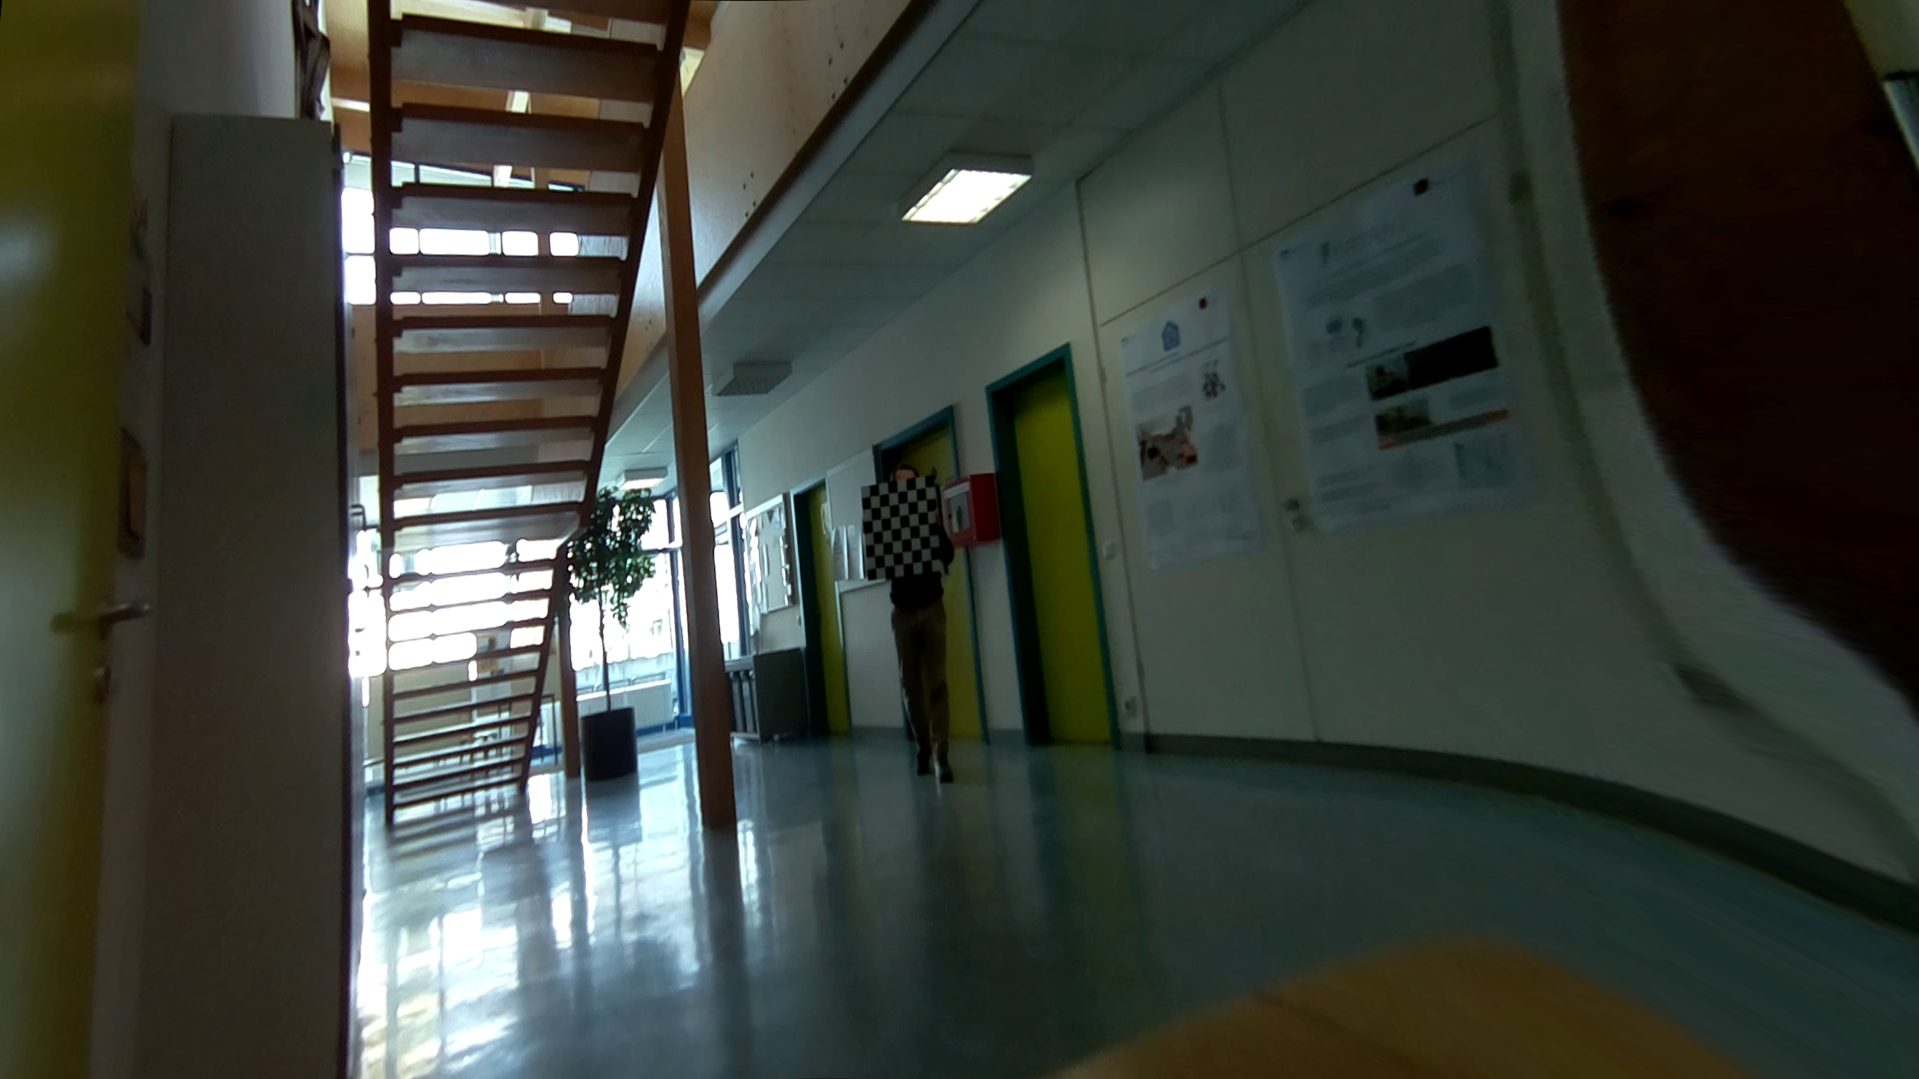
\includegraphics[width=.95\textwidth]{image/3/rec_2/525_undist.png}
     \end{minipage}
     
     \hfill
     
     \begin{minipage}[t]{0.24\textwidth}
        \centering
        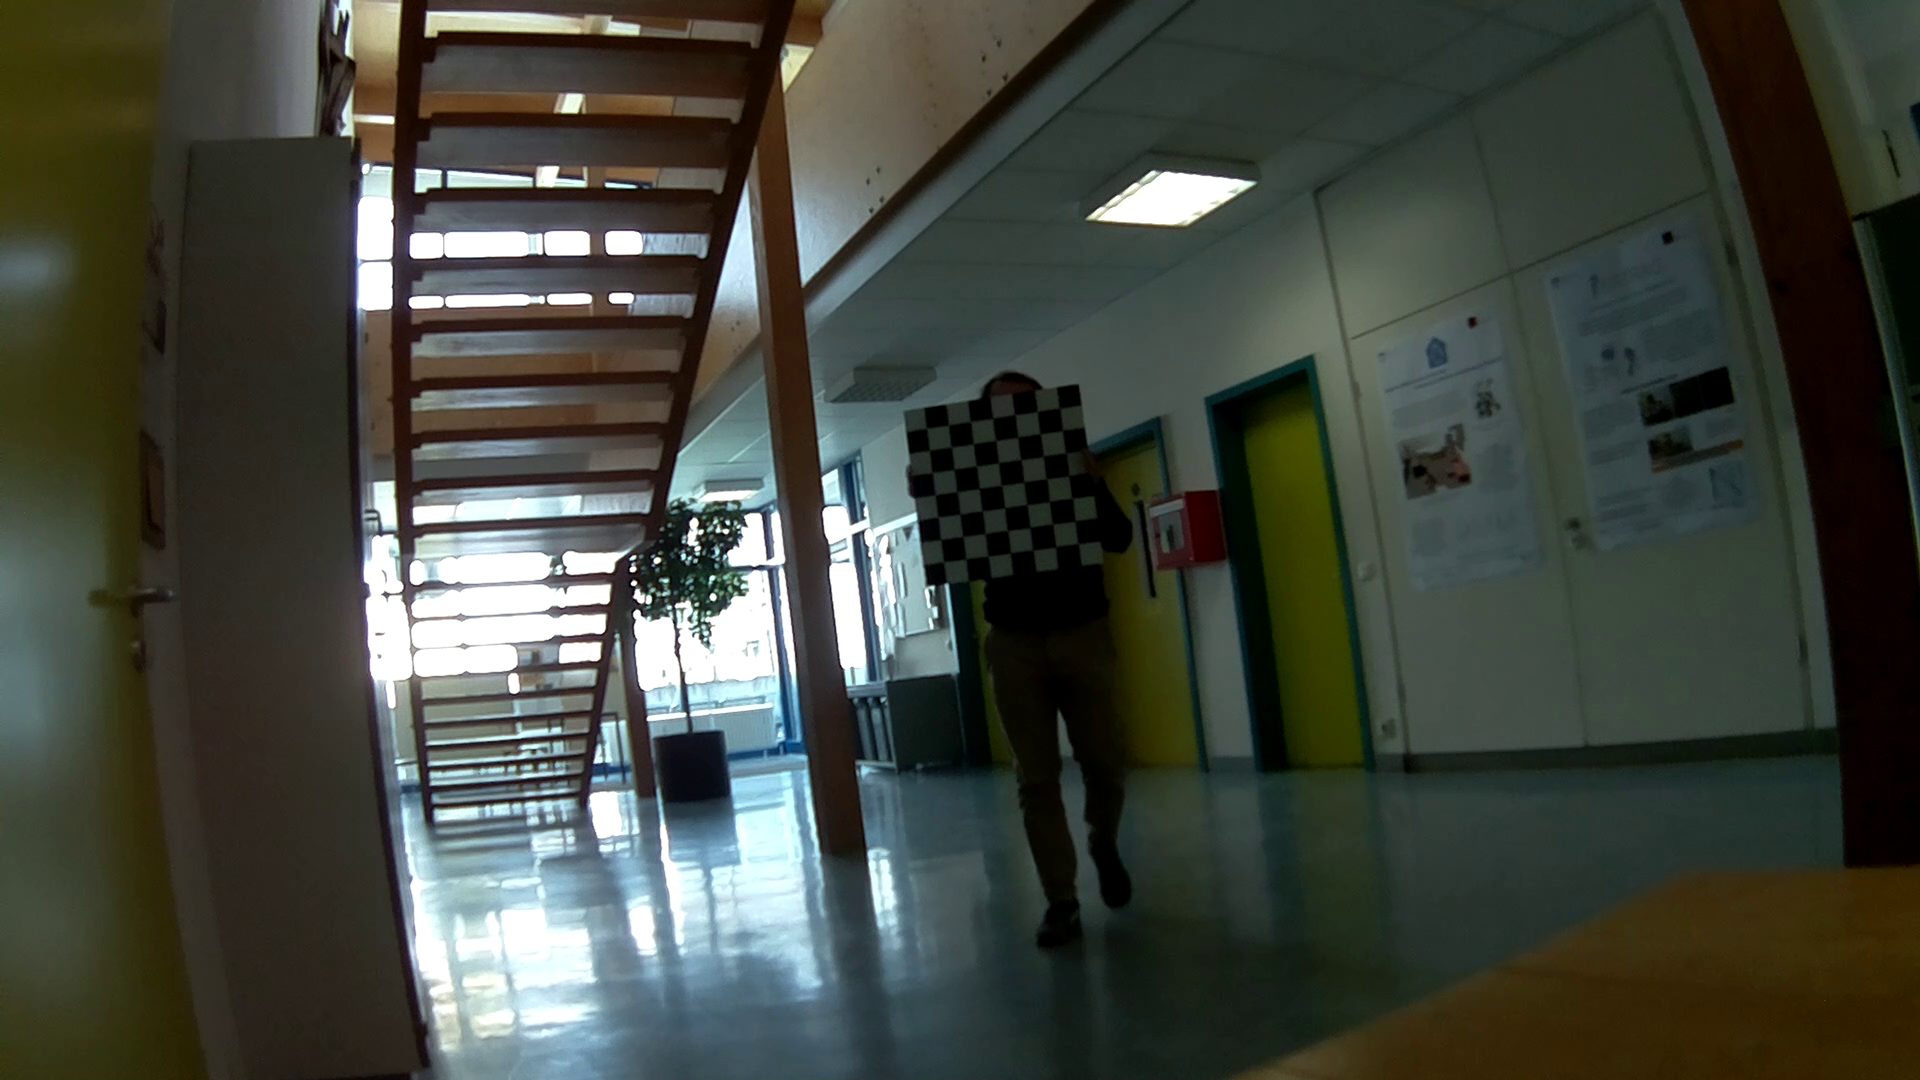
\includegraphics[width=.95\textwidth]{image/3/rec_2/622_og.png}
     \end{minipage}%
     \begin{minipage}[t]{0.24\textwidth}
        \centering
        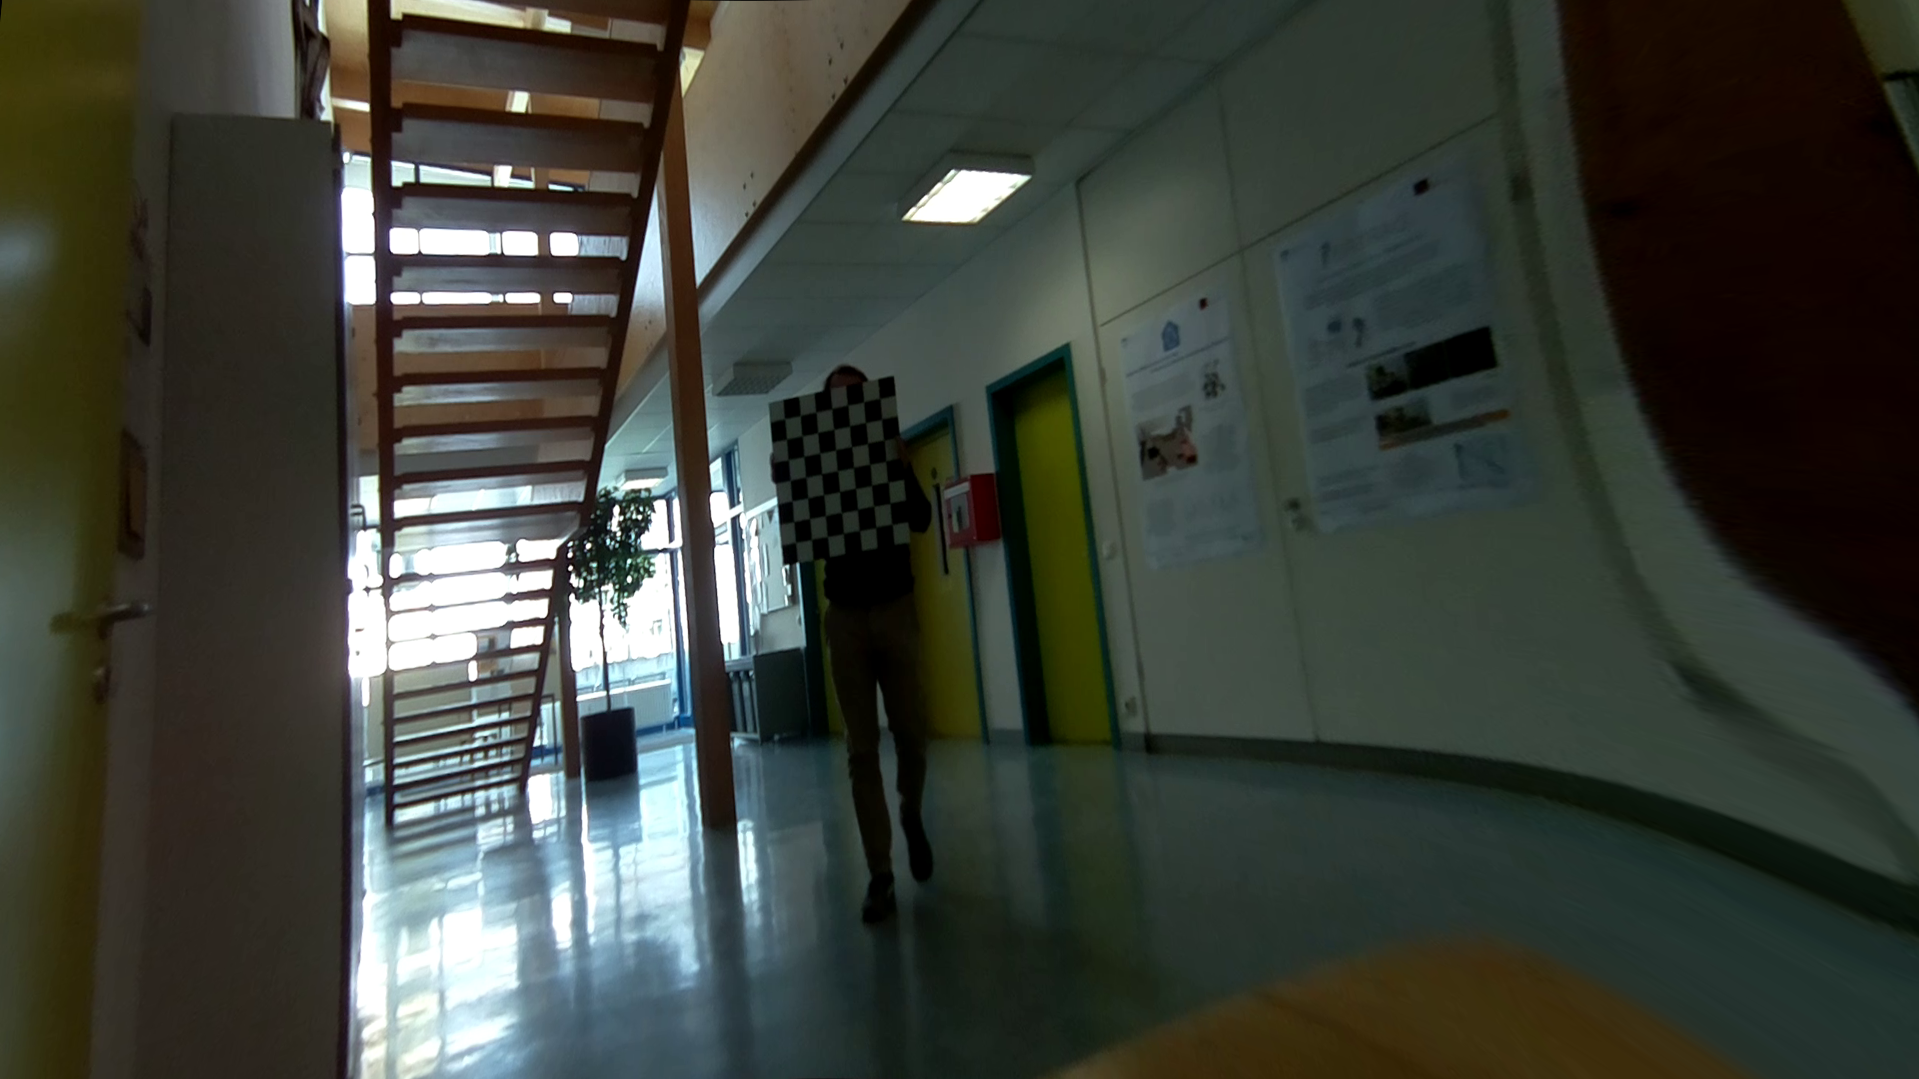
\includegraphics[width=.95\textwidth]{image/3/rec_2/622_undist.png}
     \end{minipage}
     \begin{minipage}[t]{0.24\textwidth}
        \centering
        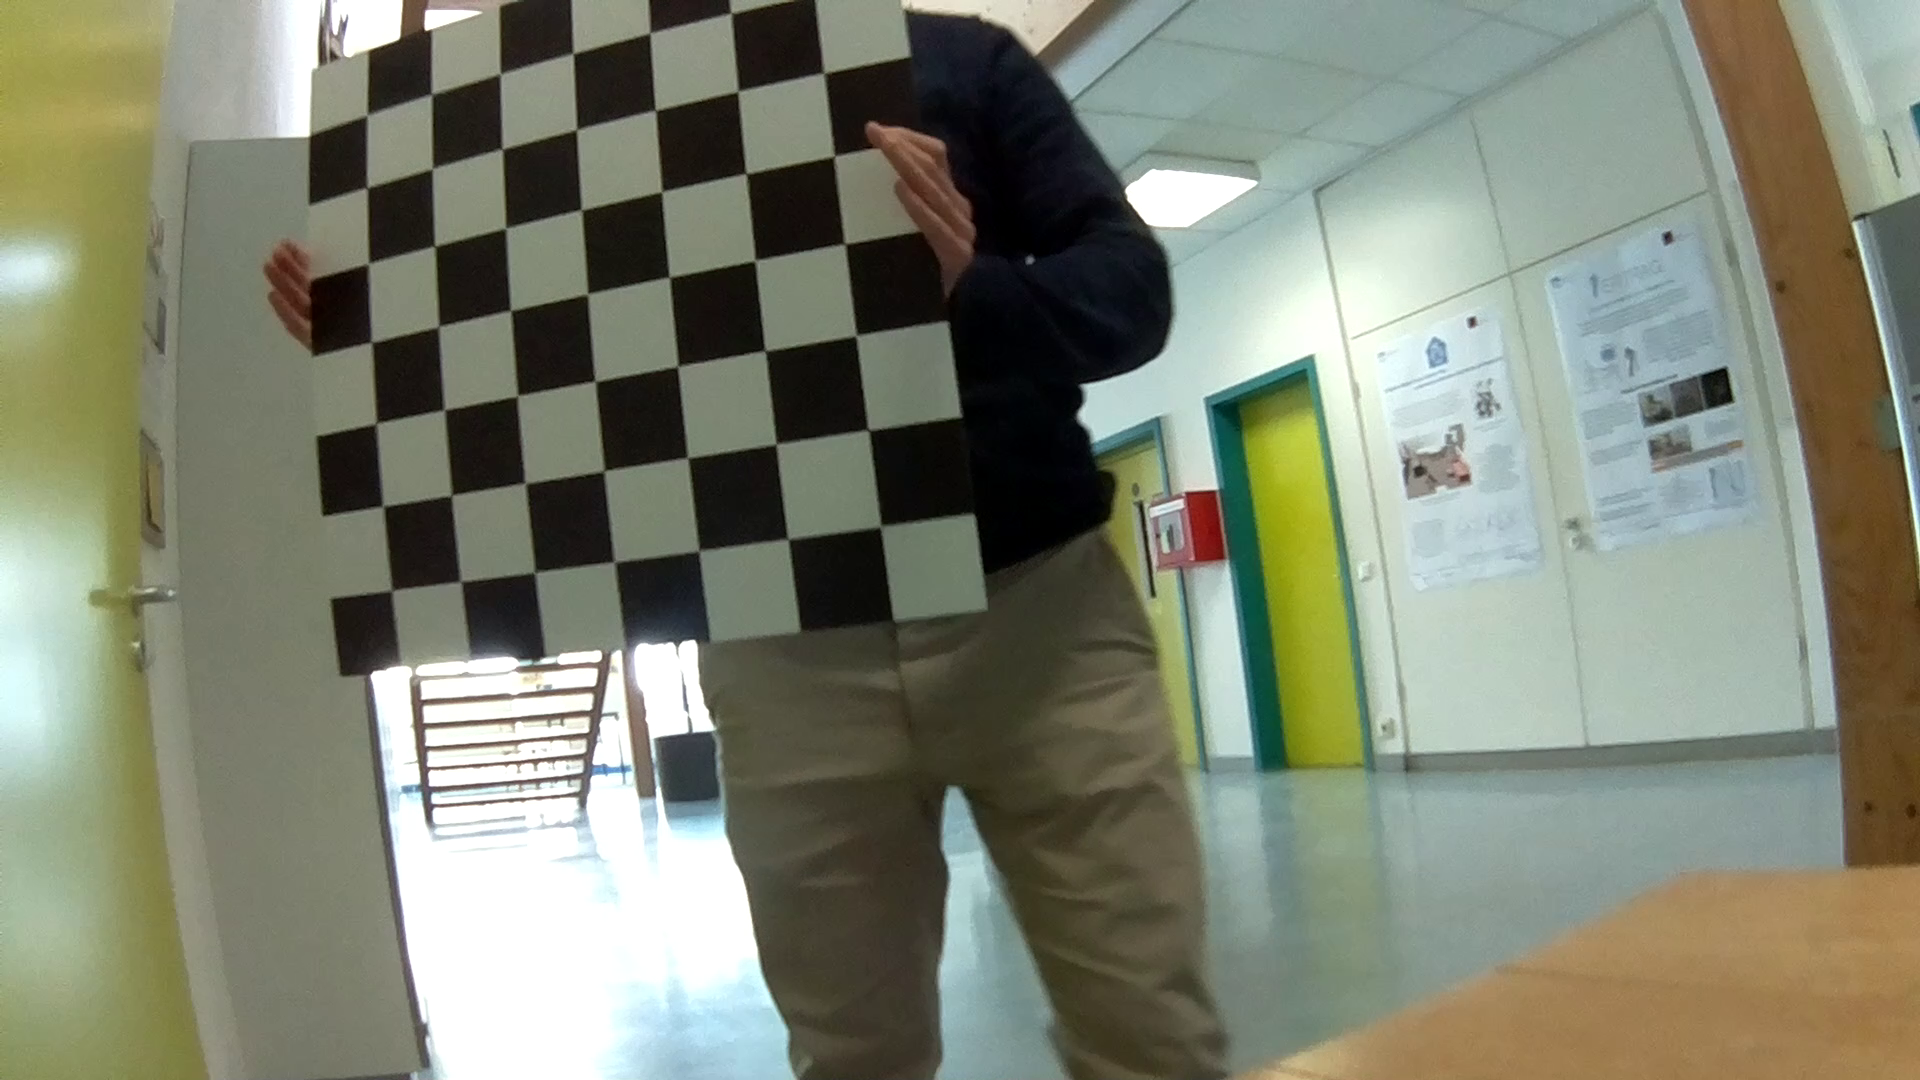
\includegraphics[width=.95\textwidth]{image/3/rec_2/737_og.png}
     \end{minipage}%
     \begin{minipage}[t]{0.24\textwidth}
        \centering
        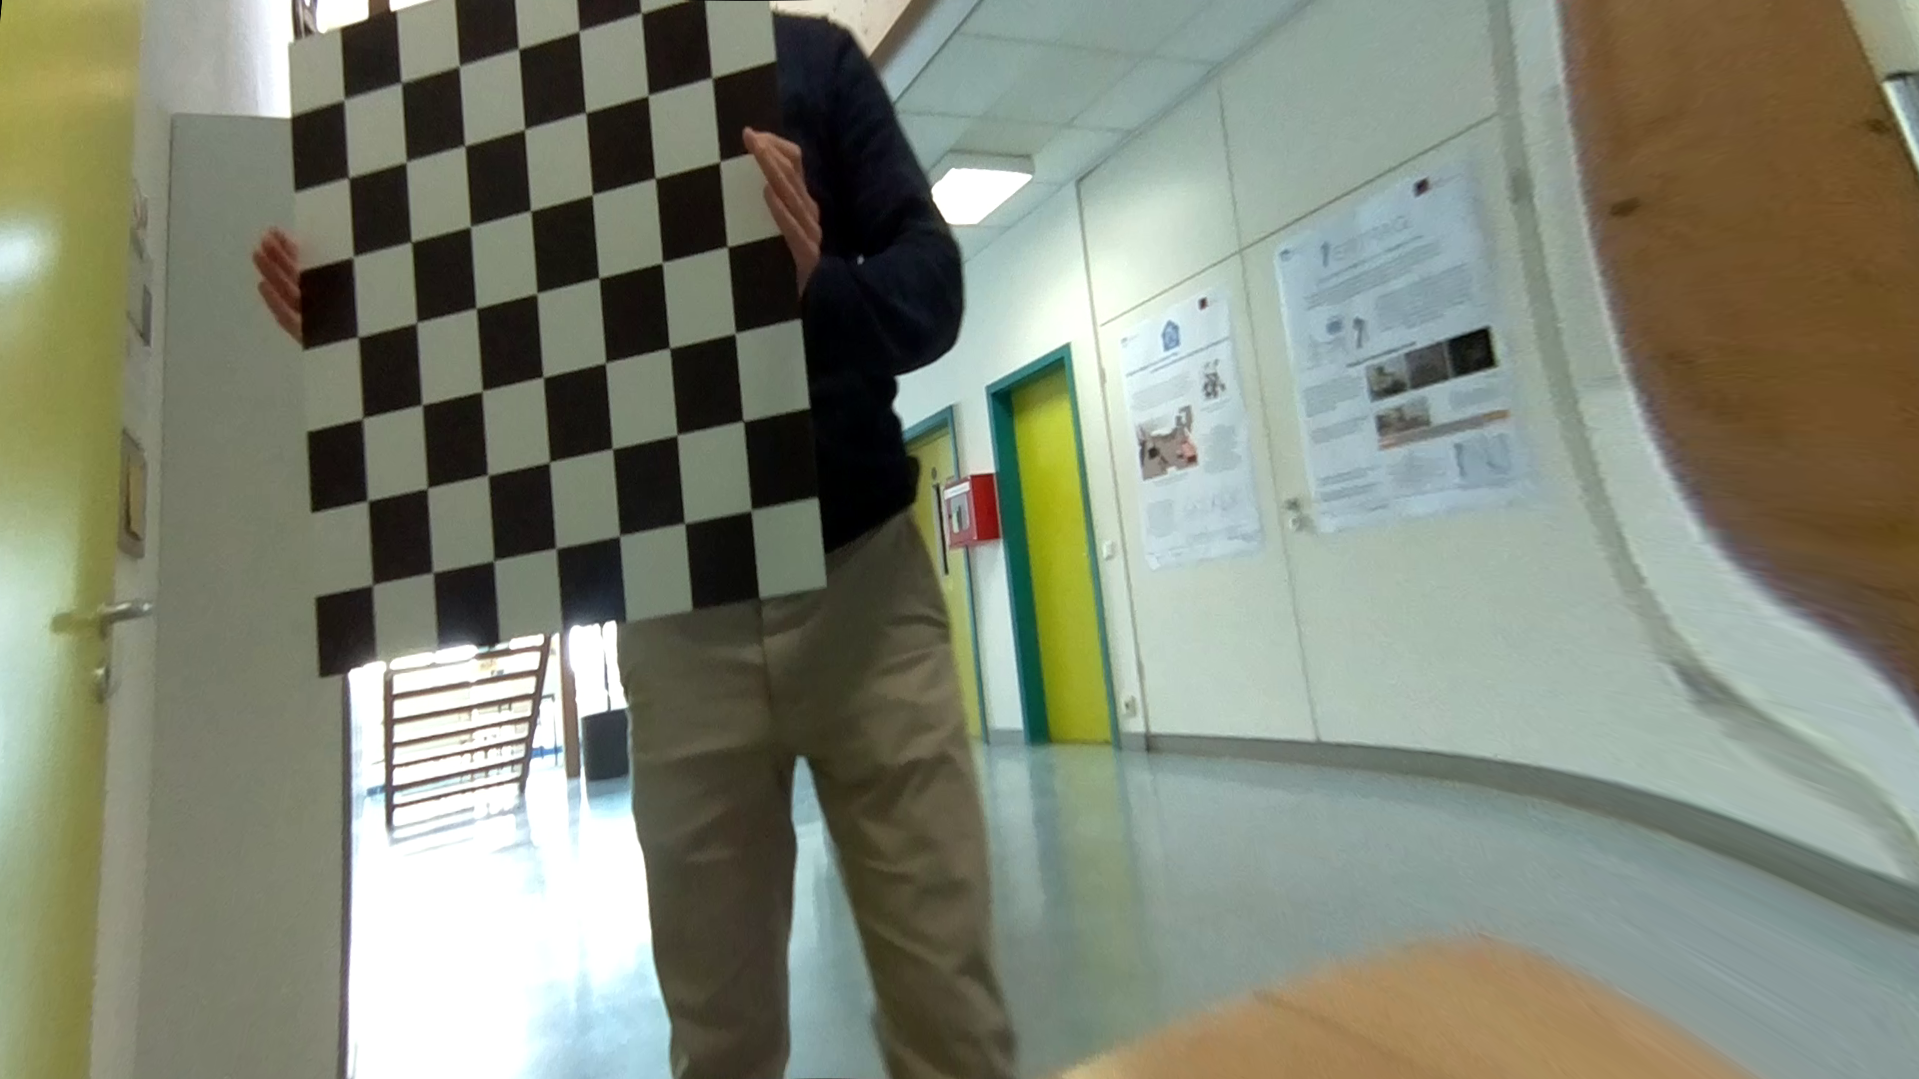
\includegraphics[width=.95\textwidth]{image/3/rec_2/737_undist.png}
     \end{minipage}
     
     \caption{Four original frames (left) from the recording \textit{checkerboard\_019.h264} with their undistorted counterpart (right)}
    \label{fig:rec_019}
\end{figure}

The undistorted images in figure \ref{fig:rec_019} do look like expected in the left and the center portion of the image. The right portion of the image however has been additionally distorted. \\

This could follow from the fact that in the 71 images used, there were none where the checkerboard was photographed on the right portion of the image. The big deviations values of $K_1$ to $K_2$ and $d_1$ to $d_2$ are an indicator. When calculation the matrix norm of both intrinsic matrices one obtains $\left \| K_1 \right \|_{\infty} = 1493.27$ and $\left \| K_2 \right \|_{\infty} = 2176.21$, which represents a 68\% difference. If the same camera in both recordings is used there should not be such a big difference.\\

This difference could also be due to the use of a different corner size, as already mentioned in chapter \ref{experiment}.\\

Because of the missing checkerboard of this portion of the image this side of the image was not included in the calculation of the intrinsic matrix and the distortion coefficients which concludes in calculation parameters unfit for this portion of the image. Additional images where the checkerboard is in the right portion of the image would fix this occurrence.